\documentclass[a4paper,12pt,french]{article}

\usepackage[cours]{../../../Style}

% Début du document
%%%%%%%%%%%%%%%%%%%
\begin{document}

\title{Fonctions: Généralités}
\author{}
\date{}
\maketitle

%\begin{FlushLeft}

\section{Définitions, notations, représentation}

\begin{defin}
Soit $D \subset \R$. On appelle fonction $f$ sur l'ensemble $D$ le processus qui à tout nombre $x \in D$ associe un unique réel noté $f(x)$. On note $\fonction f D {\R} x {f(x)}$. On dit alors que:
\begin{itemize}
\item $f(x)$ est l'image de $x$
\item $x$ est un antécédent de $f(x)$
\item $D$ est l'ensemble ( ou domaine ) de définition de $f$
\end{itemize}
\end{defin}

\begin{ex}
On définit la fonction $\fonction f {\R} {\R} x {x^2-x}$.
\begin{itemize}
\item L'image de $2$ par la fonction $f$ est $2$: $f(2)=2^2-2=2$.
\item $2$ est un antécédent de $2$ par la fonction $f$. $-1$ en est aussi un car $f(-1)=(-1)^2+1=2$.
\end{itemize}
\end{ex}

\begin{rmq}
Chaque nombre dans $D$ possède une unique image, mais plusieurs antécédents d'un même nombre peuvent exister.
\end{rmq}

\begin{defin}
Dans un repère du plan, l'ensemble des points $(x,f(x))$ pour $x \in D$ constitue la courbe de $f$. L'équation de la courbe de $f$ est $y=f(x)$ pour $x \in D$.
\end{defin}


\begin{methode}
Dans la pratique, il faut placer plusieurs points pour tracer la courbe d'une fonction le plus précisément possible. On peut s'aider d'une table de valeurs.
\end{methode}

\begin{ex} \saut
\begin{center}
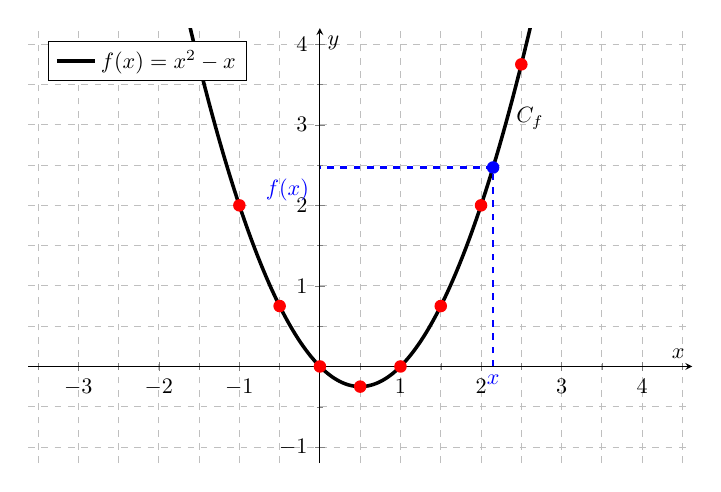
\begin{tikzpicture}[scale=0.8]
\begin{axis}[
axis x line=bottom,
axis y line = left,
axis lines=middle,
width=\linewidth,
height=0.7*\linewidth,
xmin=-2, xmax=3,
ymin=-1, ymax=4,
enlargelimits={abs=0.2},
xlabel={$x$},
ylabel={$y$},
minor x tick num=1,
minor y tick num=1,
%ytick distance=1,
grid=both,
grid style=dashed,
axis equal,
legend pos=north west,
]
\addplot[samples=101,smooth,ultra thick,domain=(-3:3),mark=none]{x^2-x} node [pos=0.85,right] {$\mathscr C_f$};
\addlegendentry{$f(x)=x^2-x$};
\pgfplotsinvokeforeach{-1.5,-1,...,2.5}{ \node[circle, minimum size=2pt,fill,color=red,inner sep=2pt] at (axis cs:#1,#1*#1-#1) {};}

\addplot +[mark=none,color=blue,style=dashed,very thick] coordinates {(2.15, 0) (2.15, 2.47)} node [pos=0,below] {$x$};
\addplot +[mark=none,color=blue,style=dashed,very thick] coordinates {(2.15, 2.47) (0, 2.47)} node [pos=1,below left=1pt] {$f(x)$};
\node[circle, minimum size=1pt,fill,color=blue,inner sep=2pt] at (axis cs:2.15,2.47) {};
%\addplot +[mark=none,color=red,style=dashed,very thick] coordinates {(-1, 0) (-1, 2)};
%\addplot +[mark=none,color=red,style=dashed,very thick] coordinates {(-1, 2) (0, 2)};
%\node[label={0:{$(0,1)$}},rectangle,fill,inner sep=2pt] at (axis cs:0,1) {};
%\node[label={[label distance=2pt]-90:{$(0,1)$}},rectangle,fill,inner sep=0pt, minimum height=0pt, minimum width=4pt] at (axis cs:1,1) {};
\end{axis}
\end{tikzpicture}
\end{center}
\end{ex}

\rem{Exos 101 -> 104 p32}
\section{Résolution graphique d'équations et d'inéquations}

\subsection{Equations}

\begin{methode} \saut
\begin{center}
\resizebox{\linewidth}{!}{
\begin{tabularx}{\textwidth}{|X|X| } \hline
\Centering{$f(x)=k$} & \Centering{$f(x)=g(x)$} \\ \hline
\Centering{
\begin{tikzpicture}[scale=1]
\begin{axis}[
axis x line=bottom,
axis y line = left,
axis lines=middle,
width=1.1*\linewidth,
height=0.8*\linewidth,
xmin=-0.5, xmax=4.5,
ymin=-1, ymax=4,
enlargelimits={abs=0.2},
xlabel={$x$},
ylabel={$y$},
%ytick distance=1,
ticks=none,
grid style=dashed,
%axis equal,
legend pos=north east,
xlabel style={at={(ticklabel* cs:0.95)},below=0.1},
]
\addplot[samples=101,smooth,ultra thick,domain=(-2:5),mark=none]{3.5*e^(-0.4*(x-2)^2)} node [pos=0.75,right] {$\mathscr C_f$};

\addplot +[mark=none,color=blue,style=dashed,very thick] coordinates {(-1,2.8) (5, 2.8)} node [pos=0.18,above right] {$k$};
\node[circle, minimum size=1pt,fill,color=blue,inner sep=2pt] at (axis cs:1.25,2.8) {};
\node[circle, minimum size=1pt,fill,color=blue,inner sep=2pt] at (axis cs:2.75,2.8) {};
\addplot +[mark=none,color=blue,style=dashed,very thick] coordinates {(1.25,0) (1.25, 2.8)} node [pos=0,below] {$x_1$};
\addplot +[mark=none,color=blue,style=dashed,very thick] coordinates {(2.75,0) (2.75, 2.8)} node [pos=0,below] {$x_2$};
%\addplot +[mark=none,color=red,style=dashed,very thick] coordinates {(-1, 0) (-1, 2)};
%\addplot +[mark=none,color=red,style=dashed,very thick] coordinates {(-1, 2) (0, 2)};
%\node[label={0:{$(0,1)$}},rectangle,fill,inner sep=2pt] at (axis cs:0,1) {};
%\node[label={[label distance=2pt]-90:{$(0,1)$}},rectangle,fill,inner sep=0pt, minimum height=0pt, minimum width=4pt] at (axis cs:1,1) {};
\end{axis}
\end{tikzpicture}}
&
\Centering{
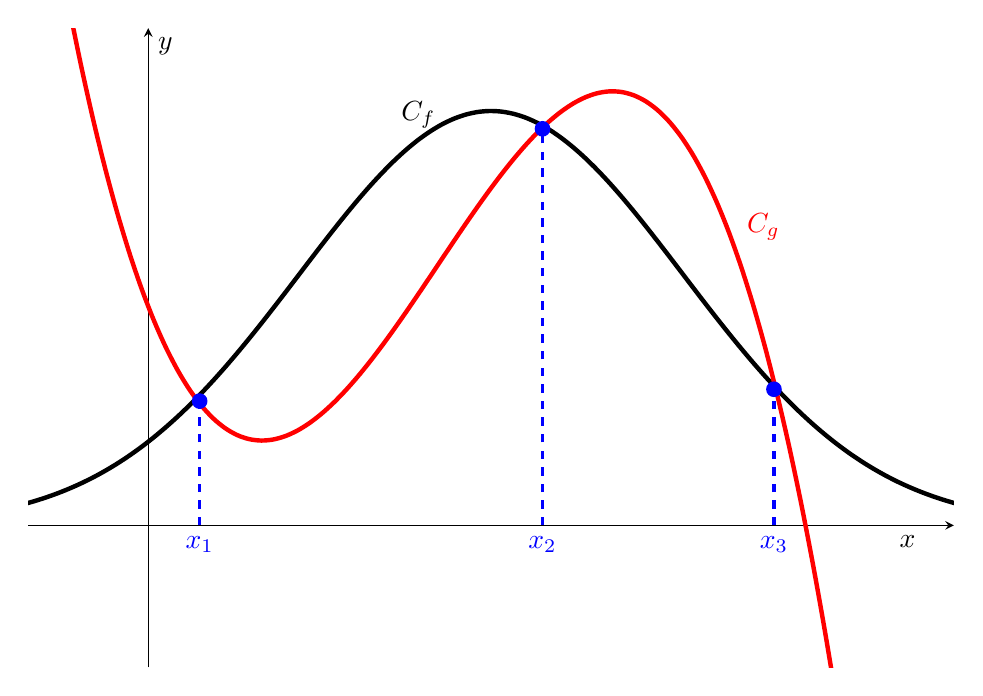
\begin{tikzpicture}[scale=1]
\begin{axis}[
axis x line=bottom,
axis y line = left,
axis lines=middle,
width=1.1*\linewidth,
height=0.8*\linewidth,
xmin=-0.5, xmax=4.5,
ymin=-1, ymax=4,
enlargelimits={abs=0.2},
xlabel={$x$},
ylabel={$y$},
ticks=none,
%ytick distance=1,
%axis equal,
yticklabel=\empty,
xticklabel=\empty,
xlabel style={at={(ticklabel* cs:0.95)},below=0.1},
]
\addplot[samples=101,smooth,ultra thick,domain=(-2:5),mark=none]{3.5*e^(-0.4*(x-2)^2)} node [pos=0.5,above] {$\mathscr C_f$};
\addplot[samples=101,smooth,ultra thick,domain=(-2:5),mark=none,color=red]{-0.69*x^3+3.49*x^2-3.72*x+1.85} node [pos=0.65,above right,color=red] {$\mathscr C_g$};

\addplot +[mark=none,color=blue,style=dashed,very thick] coordinates {(0.3,0) (0.3, 1.05)} node [pos=0,below] {$x_1$} node[pos=1,circle, minimum size=1pt,fill,inner sep=2pt] {};
\addplot +[mark=none,color=blue,style=dashed,very thick] coordinates {(2.3,0) (2.3, 3.35)} node [pos=0,below] {$x_2$} node[pos=1,circle, minimum size=1pt,fill,inner sep=2pt] {};
\addplot +[mark=none,color=blue,style=dashed,very thick] coordinates {(3.65,0) (3.65, 1.15)} node [pos=0,below] {$x_3$} node[pos=1,circle, minimum size=1pt,fill,inner sep=2pt] {};
%\addplot +[mark=none,color=red,style=dashed,very thick] coordinates {(-1, 0) (-1, 2)};
%\addplot +[mark=none,color=red,style=dashed,very thick] coordinates {(-1, 2) (0, 2)};
%\node[label={0:{$(0,1)$}},rectangle,fill,inner sep=2pt] at (axis cs:0,1) {};
%\node[label={[label distance=2pt]-90:{$(0,1)$}},rectangle,fill,inner sep=0pt, minimum height=0pt, minimum width=4pt] at (axis cs:1,1) {};
\end{axis}
\end{tikzpicture}}
\\ \hline
Résoudre l'équation $f(x)=k$ signifie trouver les antécédents de $k$ par la fonction $f$.

Cela revient donc à chercher l'abscisse des points d'intersection de la courbe avec la droite d'équation $y=k$.

Ici, l'ensemble des solution de l'équation est:$$S=\{x_1,x_2 \}$$ \vspace{-5mm}
&
Résoudre l'équation $f(x)=g(x)$ signifie trouver les nombres qui ont la même image par $f$ et $g$.

Cela revient donc à chercher l'abscisse des points d'intersection des deux courbes $\mathscr C_f$ et $\mathscr C_g$.

Ici, l'ensemble des solution de l'équation est:$$S=\{x_1,x_2,x_3 \}$$ \vspace{-5mm} \\ \hline
\end{tabularx}}
\end{center}
\end{methode}

\subsection{Inéquations}

\renewcommand\tabularxcolumn[1]{p{#1}}
\begin{methode} \saut
\begin{center}
\begin{tabularx}{\linewidth}{|X|X|X|} \hline
\Centering{$f(x)>k$} & \Centering{$f(x) \leq k$} & \Centering{$f(x)>g(x)$} \\ \hline
\multicolumn{2}{|c|}{
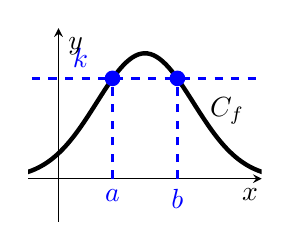
\begin{tikzpicture}[scale=1]
\begin{axis}[
axis x line=bottom,
axis y line = left,
axis lines=middle,
width=0.375*\linewidth,
height=0.333*\linewidth,
xmin=-0.5, xmax=4.5,
ymin=-1, ymax=4,
enlargelimits={abs=0.2},
xlabel={$x$},
ylabel={$y$},
%ytick distance=1,
ticks=none,
grid style=dashed,
%axis equal,
legend pos=north east,
xlabel style={at={(ticklabel* cs:0.95)},below=0.1},
]
\addplot[samples=101,smooth,ultra thick,domain=(-2:5),mark=none]{3.5*e^(-0.4*(x-2)^2)} node [pos=0.75,right] {$\mathscr C_f$};

\addplot +[mark=none,color=blue,style=dashed,very thick] coordinates {(-1,2.8) (5, 2.8)} node [pos=0.18,above right] {$k$};
\node[circle, minimum size=1pt,fill,color=blue,inner sep=2pt] at (axis cs:1.25,2.8) {};
\node[circle, minimum size=1pt,fill,color=blue,inner sep=2pt] at (axis cs:2.75,2.8) {};
\addplot +[mark=none,color=blue,style=dashed,very thick] coordinates {(1.25,0) (1.25, 2.8)} node [pos=0,below] {$a$};
\addplot +[mark=none,color=blue,style=dashed,very thick] coordinates {(2.75,0) (2.75, 2.8)} node [pos=0,below] {$b$};
%\addplot +[mark=none,color=red,style=dashed,very thick] coordinates {(-1, 0) (-1, 2)};
%\addplot +[mark=none,color=red,style=dashed,very thick] coordinates {(-1, 2) (0, 2)};
%\node[label={0:{$(0,1)$}},rectangle,fill,inner sep=2pt] at (axis cs:0,1) {};
%\node[label={[label distance=2pt]-90:{$(0,1)$}},rectangle,fill,inner sep=0pt, minimum height=0pt, minimum width=4pt] at (axis cs:1,1) {};
\end{axis}
\end{tikzpicture}}
&
\Centering{
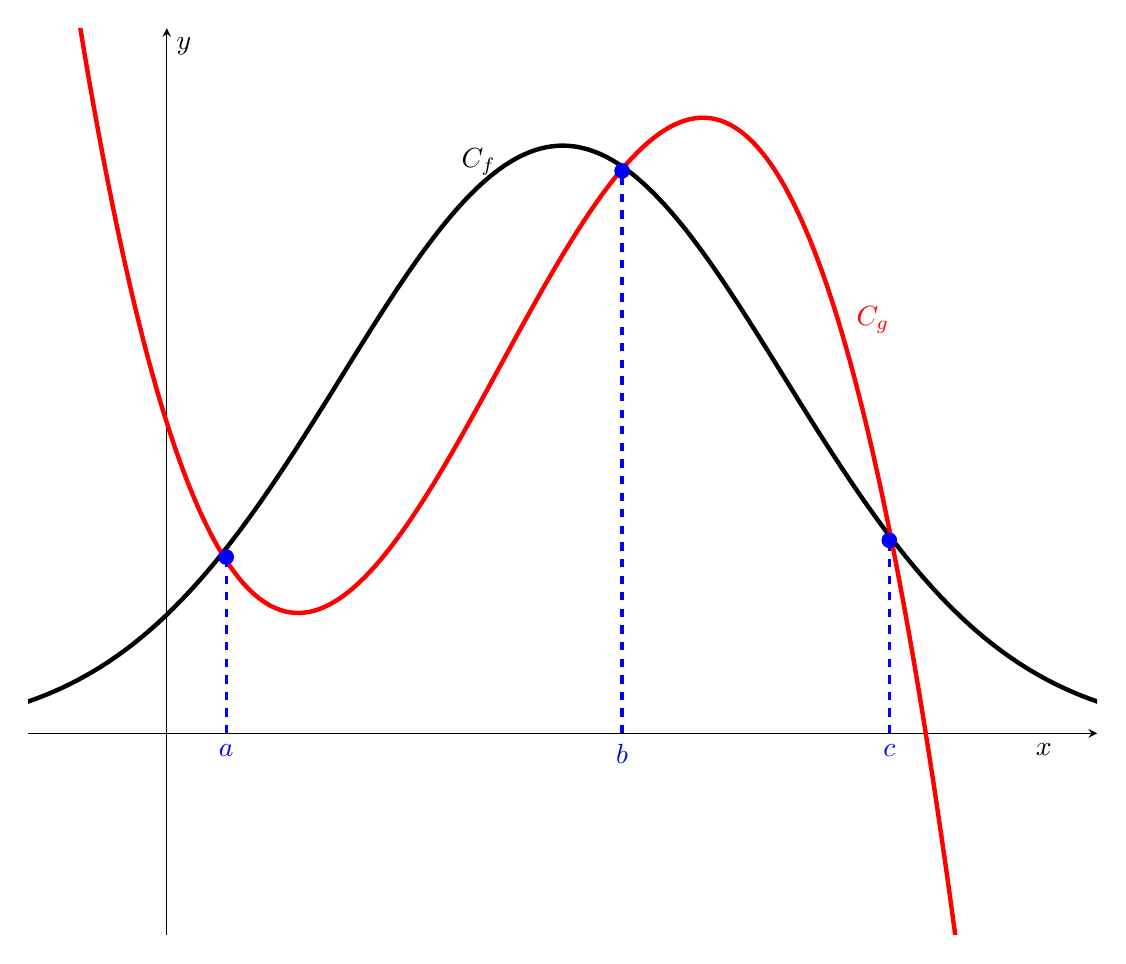
\begin{tikzpicture}[scale=1]
\begin{axis}[
axis x line=bottom,
axis y line = left,
axis lines=middle,
width=1.25*\linewidth,
height=1.08*\linewidth,
xmin=-0.5, xmax=4.5,
ymin=-1, ymax=4,
enlargelimits={abs=0.2},
xlabel={$x$},
ylabel={$y$},
ticks=none,
%ytick distance=1,
%axis equal,
yticklabel=\empty,
xticklabel=\empty,
xlabel style={at={(ticklabel* cs:0.95)},below=0.1},
]
\addplot[samples=101,smooth,ultra thick,domain=(-2:5),mark=none]{3.5*e^(-0.4*(x-2)^2)} node [pos=0.5,above] {$\mathscr C_f$};
\addplot[samples=101,smooth,ultra thick,domain=(-2:5),mark=none,color=red]{-0.69*x^3+3.49*x^2-3.72*x+1.85} node [pos=0.65,above right,color=red] {$\mathscr C_g$};

\addplot +[mark=none,color=blue,style=dashed,very thick] coordinates {(0.3,0) (0.3, 1.05)} node [pos=0,below] {$a$} node[pos=1,circle, minimum size=1pt,fill,inner sep=2pt] {};
\addplot +[mark=none,color=blue,style=dashed,very thick] coordinates {(2.3,0) (2.3, 3.35)} node [pos=0,below] {$b$} node[pos=1,circle, minimum size=1pt,fill,inner sep=2pt] {};
\addplot +[mark=none,color=blue,style=dashed,very thick] coordinates {(3.65,0) (3.65, 1.15)} node [pos=0,below] {$c$} node[pos=1,circle, minimum size=1pt,fill,inner sep=2pt] {};
%\addplot +[mark=none,color=red,style=dashed,very thick] coordinates {(-1, 0) (-1, 2)};
%\addplot +[mark=none,color=red,style=dashed,very thick] coordinates {(-1, 2) (0, 2)};
%\node[label={0:{$(0,1)$}},rectangle,fill,inner sep=2pt] at (axis cs:0,1) {};
%\node[label={[label distance=2pt]-90:{$(0,1)$}},rectangle,fill,inner sep=0pt, minimum height=0pt, minimum width=4pt] at (axis cs:1,1) {};
\end{axis}
\end{tikzpicture}}
\\ \hline
Résoudre l'inéquation $f(x)>k$ signifie trouver les nombres qui ont une image supérieure à $k$.

Cela revient donc à chercher l'abscisse des points de la courbe se situant "au dessus" de la droite d'équation $y=k$.

Ici, l'ensemble des solution de l'inéquation est:$$S=\left] a;b \right[$$ \vspace{-5mm}
&
Résoudre l'inéquation $f(x) \leq k$ signifie trouver les nombres qui ont une image inférieure à $k$.

Cela revient donc à chercher l'abscisse des points de la courbe se situant "en dessous" de la droite d'équation $y=k$.

Ici, l'ensemble des solution de l'inéquation est:$$S=\left] - \infty;a \right] \cup \left[ b ; + \infty \right[$$ \vspace{-5mm}
&
Résoudre l'inéquation $f(x) > g(x)$ signifie trouver les nombres dont l'image par $f$ est supérieure à l'image par $g$.
Cela revient à chercher l'abscisse des points de $\mathscr C_f$ situés "au dessus" des points de $\mathscr C_g$.

Ici, l'ensemble des solutions de l'inéquation est:$$S=\left] - \infty;a \right[ \cup \left] b ; c \right[$$ \vspace{-5mm} \\ \hline
\end{tabularx}
\end{center}
\end{methode}
\renewcommand\tabularxcolumn[1]{m{#1}}
\rem{Exos 105 -> 110 p32}

\section{Etudes de fonctions}

\subsection{Etude des variations}

\begin{defin}
Soit $f$ définie sur un intervalle $I$.
\begin{itemize}
\item On dit que $f$ est croissante sur I si lorsque la variable augmente dans $I$, les images augmentent aussi : Pour $x,y \in I$, si $x \leq y$ alors $f(x) \leq f(y)$.:
\item On dit que $f$ est décroissante sur I si lorsque la variable augmente dans $I$, les images diminuent: Pour $x,y \in I$, si $x \leq y$ alors $f(x) \geq f(y)$.
\end{itemize}
\end{defin}

\begin{methode}
Dresser le tableau de variations d'une fonction $f$, c'est indiquer sur quels intervalles la fonction $f$ est croissante, décroissante ou constante.
\end{methode}

\begin{ex} \saut
\compo[0.45]{
\begin{center}
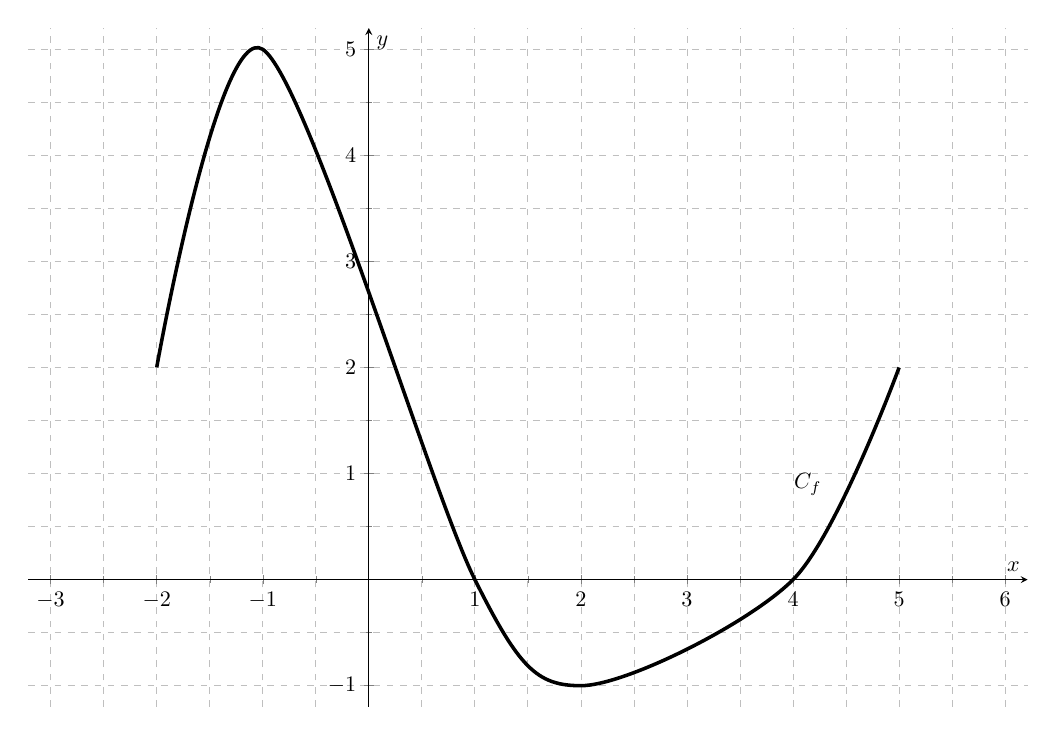
\begin{tikzpicture}[scale=0.8]
\begin{axis}[
axis x line=bottom,
axis y line = left,
axis lines=middle,
width=2\linewidth,
height=1.4*\linewidth,
xmin=-2, xmax=5,
ymin=-1, ymax=5,
enlargelimits={abs=0.2},
xlabel={$x$},
ylabel={$y$},
minor x tick num=1,
minor y tick num=1,
%ytick distance=1,
grid=both,
grid style=dashed,
axis equal,
legend pos=north east,
scale=0.7
]
\addplot[samples=101,smooth,ultra thick,domain=(0:4),mark=none] plot coordinates {(-2,2) (-1,5) (1,0) (2,-1) (4,0) (5,2)} node [pos=0.9,above left] {$\mathscr C_f$};

\end{axis}
\end{tikzpicture}
\end{center}
}
{

%:-+-+-+-+- Engendré par : http://math.et.info.free.fr/TikZ/TableauxVariations/
\begin{center}
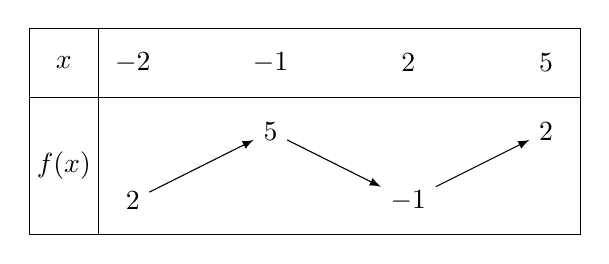
\begin{tikzpicture}[scale=0.875]

% Styles 
\tikzstyle{cadre}=[thin]
\tikzstyle{fleche}=[->,>=latex,thin]
\tikzstyle{nondefini}=[lightgray]
% Dimensions Modifiables
\def\Lrg{1}
\def\HtX{1}
\def\HtY{0.5}
% Dimensions Calculées
\def\lignex{-0.5*\HtX}
\def\lignef{-1.5*\HtX}
\def\separateur{-0.5*\Lrg}
% Largeur du tableau
\def\gauche{-1.5*\Lrg}
\def\droite{6.5*\Lrg}
% Hauteur du tableau
\def\haut{0.5*\HtX}
\def\bas{-1.5*\HtX-2*\HtY}
% Ligne de l'abscisse : x
\node at (-1*\Lrg,0) {$x$};
\node at (0*\Lrg,0) {$-2$};
\node at (2*\Lrg,0) {$-1$};
\node at (4*\Lrg,0) {$2$};
\node at (6*\Lrg,0) {$5$};
% Ligne de la fonction : f(x)
\node  at (-1*\Lrg,{-1*\HtX+(-1)*\HtY}) {$f(x)$};
\node (f1) at (0*\Lrg,{-1*\HtX+(-2)*\HtY}) {$2$};
\node (f2) at (2*\Lrg,{-1*\HtX+(0)*\HtY}) {$5$};
\node (f3) at (4*\Lrg,{-1*\HtX+(-2)*\HtY}) {$-1$};
\node (f4) at (6*\Lrg,{-1*\HtX+(0)*\HtY}) {$2$};
% Flèches
\draw[fleche] (f1) -- (f2);
\draw[fleche] (f2) -- (f3);
\draw[fleche] (f3) -- (f4);
% Encadrement
\draw[cadre] (\separateur,\haut) -- (\separateur,\bas);
\draw[cadre] (\gauche,\haut) rectangle  (\droite,\bas);
\draw[cadre] (\gauche,\lignex) -- (\droite,\lignex);
\end{tikzpicture}
\end{center}
%:-+-+-+-+- Fin

%:>>>>> code du tableau à ré-injecter
%[
%	["x", "f'(x)", "f(x)"],
%	["-2", "", "+", "2"],
%	["-1", "", "-", "5"],
%	["2", "", "+", "-1"],
%	["5", "", "?", "2"]
%]
}
\end{ex}

\subsection{Etude du signe}

\begin{methode}
Dresser le tableau de signes d'une fonction $f$, c'est indiquer sur quels intervalles la fonction est négative, positive ou nulle.

Avec la même fonction que précédemment, on obtient:
%:-+-+-+-+- Engendré par : http://math.et.info.free.fr/TikZ/TableauxVariations/
\begin{center}
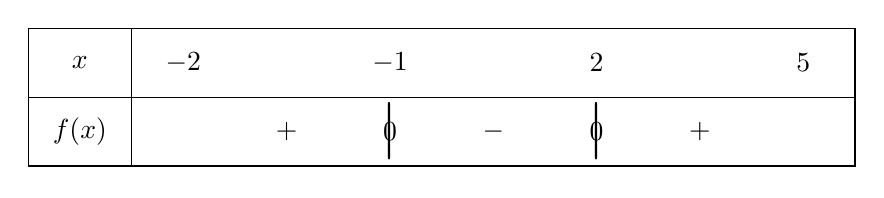
\begin{tikzpicture}[scale=0.875]
% Styles 
\tikzstyle{cadre}=[thin]
\tikzstyle{fleche}=[->,>=latex,thin]
\tikzstyle{nondefini}=[lightgray]
% Dimensions Modifiables
\def\Lrg{1.5}
\def\HtX{1}
\def\HtY{0.5}
% Dimensions Calculées
\def\lignex{-0.5*\HtX}
\def\lignef{-1.5*\HtX}
\def\separateur{-0.5*\Lrg}
% Largeur du tableau
\def\gauche{-1.5*\Lrg}
\def\droite{6.5*\Lrg}
% Hauteur du tableau
\def\haut{0.5*\HtX}
\def\bas{-2.5*\HtX-2*\HtY}
% Ligne de l'abscisse : x
\node at (-1*\Lrg,0) {$x$};
\node at (0*\Lrg,0) {$-2$};
\node at (2*\Lrg,0) {$-1$};
\node at (4*\Lrg,0) {$2$};
\node at (6*\Lrg,0) {$5$};
% Ligne de la dérivée : f'(x)
\node at (-1*\Lrg,-1*\HtX) {$f(x)$};
\node at (1*\Lrg,-1*\HtX) {$+$};
\node at (2*\Lrg,-1*\HtX) {$0$};
\node at (2*\Lrg,-1*\HtX) {\huge{$\vert$}};
\node at (3*\Lrg,-1*\HtX) {$-$};
\node at (4*\Lrg,-1*\HtX) {$0$};
\node at (4*\Lrg,-1*\HtX) {\huge{$\vert$}};
\node at (5*\Lrg,-1*\HtX) {$+$};
% Ligne de la fonction : f(x)
% Encadrement
\draw[cadre] (\separateur,\haut) -- (\separateur, \lignef);
\draw[cadre] (\gauche,\haut) rectangle  (\droite, \lignef);
\draw[cadre] (\gauche,\lignex) -- (\droite,\lignex);
\end{tikzpicture}
\end{center}
%:-+-+-+-+- Fin

%:>>>>> code du tableau à ré-injecter
%[
%	["x", "f(x)", ""],
%	["-2", "", "+", ""],
%	["-1", "0", "-", ""],
%	["2", "0", "+", ""],
%	["5", "", "?", ""]
%]

\end{methode}

\rem{Exos 111 -> 114 p32}

\section{Taux de variation d'une fonction}

\begin{defin}
Le taux de variation entre $a$ et $b$ d'une fonction $f$ définie sur un intervalle $I$ est le quotient $\dfrac{f(b)-f(a)} {b-a}$ pour $a$ et $b$ distincts et appartenant à $I$.
\end{defin}

\begin{rmq}
Ce taux correspond au coefficient directeur de la droite passant par les points de la courbe de $f$ d'abscisses respectives $a$ et $b$.

\begin{center}
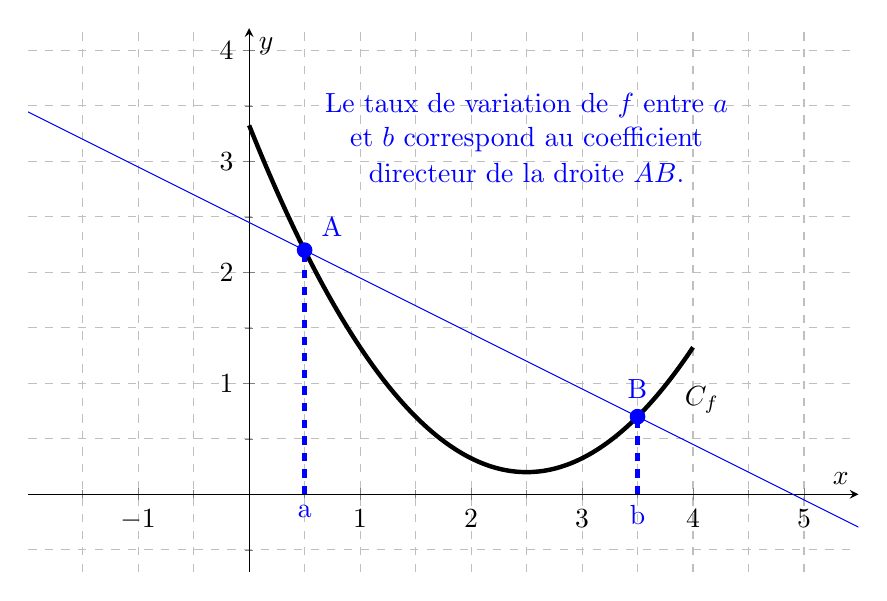
\begin{tikzpicture}[scale=1]
\begin{axis}[
axis x line=bottom,
axis y line = left,
axis lines=middle,
width=\linewidth,
height=0.7*\linewidth,
xmin=-0.5, xmax=4,
ymin=-0.5, ymax=4,
enlargelimits={abs=0.2},
xlabel={$x$},
ylabel={$y$},
minor x tick num=1,
minor y tick num=1,
%ytick distance=1,
grid=both,
grid style=dashed,
axis equal,
legend pos=north east,
]
\addplot[samples=101,smooth,ultra thick,domain=(0:4),mark=none]{0.5*(x-2.5)^2+0.2} node [pos=0.95,below right] {$\mathscr C_f$};

\node[color=blue,circle,minimum size=1pt,fill,inner sep=2pt,label={[blue]B}] (B) at (3.5,0.7) {};
\node[color=blue,circle,minimum size=1pt,fill,inner sep=2pt,label={[blue]30:A}] (A) at (0.5,2.2) {};
\draw [color=blue,shorten >=-5cm,shorten <=-5cm] (A)--(B);
\node[color=blue] at (2.5,3.5) {Le taux de variation de $f$ entre $a$};
\node[color=blue] at (2.5,3.2) {et $b$ correspond au coefficient};
\node[color=blue] at (2.5,2.9) {directeur de la droite $AB$.};
\addplot +[mark=none,color=blue,style=dashed,ultra thick] coordinates {(0.5,0) (0.5, 2.2)} node[pos=0,below] {a};
\addplot +[mark=none,color=blue,style=dashed,ultra thick] coordinates {(3.5,0) (3.5, 0.7)} node[pos=0,below] {b};

\end{axis}
\end{tikzpicture}
\end{center}
\end{rmq}

\begin{ex}
Le taux de variation entre $-1$ et $3$ de la fonction $\fonction f {\R} {\R} x {x^2-x}$ est: $$\dfrac{f(3)-f(-1)}{3-(-1)}=\dfrac{6-2}{4}=1$$
\end{ex}

\begin{prop}
Soit $f$ une fonction définie sur un intervalle $I$. $f$ est monotone (c'est-à-dire croissante ou bien décroissante sur $I$) si et seulement si le signe du taux de variation entre deux nombres quelconques de $I$ est constant.

En pratique:
\begin{itemize}
\item Un taux de variation toujours positif sur $I$ équivaut à $f$ croissante sur $I$.
\item Un taux de variation toujours négatif sur $I$ équivaut à $f$ décroissante sur $I$.
\item Un taux de variation toujours nul sur $I$ équivaut à $f$ constante sur $I$.
\end{itemize}
\end{prop}

\rem{Exos 15,16p120 et 40 -> 44 p122}

%\end{FlushLeft}

\begin{comment}

%Exemples de graphes

\begin{center}
\begin{tikzpicture}
\begin{axis}[
axis x line=bottom,
axis y line = left,
axis lines=middle,
width=\linewidth,
xmin=-5, xmax=5,
%ymin=-5, ymax=20,
%enlargelimits=true,
%xlabel=$x$,
ylabel={$f(x) = x^2$},
minor x tick num=1,
minor y tick num=4,
%ytick distance=1,
grid=major,
grid style=dashed,
axis equal,
]
\addplot[smooth]{x^2};
\addplot[smooth,domain=0:14]{ln(x)};

\end{axis}
\end{tikzpicture}
\end{center}

\begin{center}
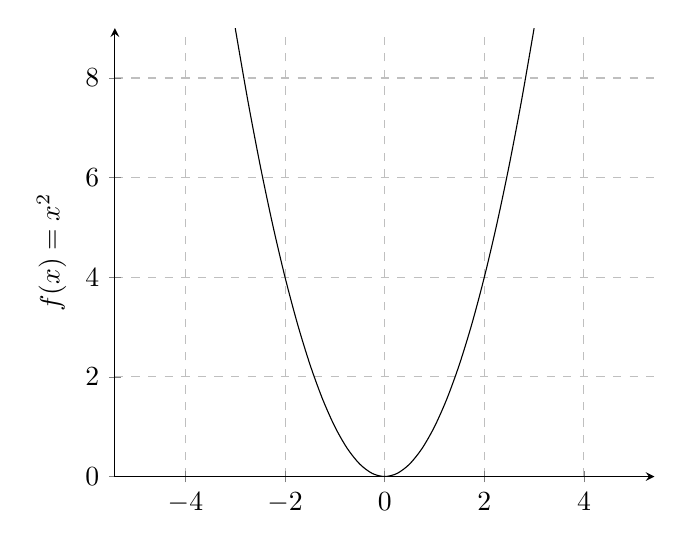
\begin{tikzpicture}
\begin{axis}[
axis x line=bottom,
axis y line = left,
%enlargelimits=true,
%xlabel=$x$,
ylabel={$f(x) = x^2$},
grid=major,
grid style=dashed,
axis equal,
]
%
use TeX as calculator:
\addplot[domain=-3:3,smooth] {x^2};
\end{axis}
\end{tikzpicture}
\end{center}

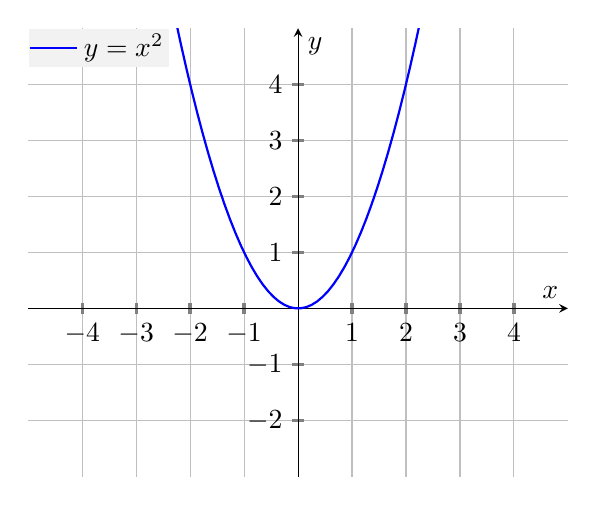
\begin{tikzpicture}
\begin{axis}[
  axis lines=middle,
  grid=major,
  xmin=-5,
  xmax=5,
  ymin=-3,
  ymax=5,
  xlabel=$x$,
  ylabel=$y$,
  xtick={-4,-3,...,4},
  ytick={-2,-1,...,4},
  tick style={very thick},
  legend style={
  at={(rel axis cs:0,1)},
  anchor=north west,draw=none,inner sep=0pt,fill=gray!10}
]
\addplot[blue,thick,samples=100] {x^2};
\addlegendentry{$y=x^2$}
\end{axis}
\end{tikzpicture}

\begin{center}
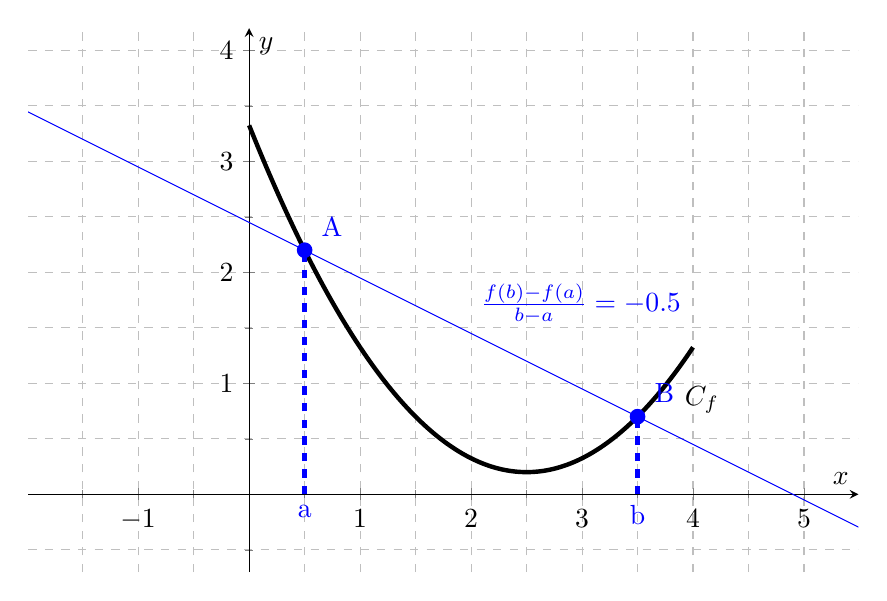
\begin{tikzpicture}[scale=1]
\begin{axis}[
axis x line=bottom,
axis y line = left,
axis lines=middle,
width=\linewidth,
height=0.7*\linewidth,
xmin=-0.5, xmax=4,
ymin=-0.5, ymax=4,
enlargelimits={abs=0.2},
xlabel={$x$},
ylabel={$y$},
minor x tick num=1,
minor y tick num=1,
%ytick distance=1,
grid=both,
grid style=dashed,
axis equal,
legend pos=north east,
]
\addplot[samples=101,smooth,ultra thick,domain=(0:4),mark=none]{0.5*(x-2.5)^2+0.2} node [pos=0.95,below right] {$\mathscr C_f$};

\node[color=blue,circle,minimum size=1pt,fill,inner sep=2pt,label={[blue]30:B}] (B) at (3.5,0.7) {};
\node[color=blue,circle,minimum size=1pt,fill,inner sep=2pt,label={[blue]30:A}] (A) at (0.5,2.2) {};
\draw [color=blue,shorten >=-5cm,shorten <=-5cm] (A)--(B) node[pos=0.5,above right] {$\frac{f(b)-f(a)} {b-a}=-0.5$};
%\addplot +[mark=none,color=blue,thick,domain=-10:10] {-0.5*x+2.45};
\addplot +[mark=none,color=blue,style=dashed,ultra thick] coordinates {(0.5,0) (0.5, 2.2)} node[pos=0,below] {a};
\addplot +[mark=none,color=blue,style=dashed,ultra thick] coordinates {(3.5,0) (3.5, 0.7)} node[pos=0,below] {b};
%\addplot +[mark=none,color=blue] coordinates {(0.5,2.2) (3.5, 0.7)} node[pos=0,circle, minimum size=1pt,fill,inner sep=2pt] {} node[pos=0,above right] {A} node[pos=1,circle, minimum size=1pt,fill,inner sep=2pt] {} node[pos=1,above] {B} node[pos=0.5,above right] {$\frac{f(b)-f(a)} {b-a}=-0.5$};
%\draw [green, ->] (2, 2) -- ++(axis direction cs:0,-1.5);
%\addlegendentry{$f(x)=x^2-x+1$};
%\pgfplotsinvokeforeach{-1.5,-1,...,2.5}{ \node[circle, minimum size=2pt,fill,color=red,inner sep=2pt] at (axis cs:#1,#1*#1-#1) {};}

%\addplot +[mark=none,color=blue,style=dashed,very thick] coordinates {(2.15, 0) (2.15, 2.47)} node [pos=0,below right] {$x$};
%\addplot +[mark=none,color=blue,style=dashed,very thick] coordinates {(2.15, 2.47) (0, 2.47)} node [pos=1,left] {$f(x)$};
%\node[circle, minimum size=1pt,fill,color=blue,inner sep=2pt] at (axis cs:2.15,2.47) {};
%\addplot +[mark=none,color=red,style=dashed,very thick] coordinates {(-1, 0) (-1, 2)};
%\addplot +[mark=none,color=red,style=dashed,very thick] coordinates {(-1, 2) (0, 2)};
%\node[label={0:{$(0,1)$}},rectangle,fill,inner sep=2pt] at (axis cs:0,1) {};
%\node[label={[label distance=2pt]-90:{$(0,1)$}},rectangle,fill,inner sep=0pt, minimum height=0pt, minimum width=4pt] at (axis cs:1,1) {};
\end{axis}
\end{tikzpicture}
\end{center}

\end{comment}


\end{document}
